\documentclass{article}
\usepackage{graphicx} % Required for inserting images
\usepackage{blindtext}
\usepackage{hyperref}
\usepackage{amsmath}

\title{21-10-2024}
\author{Samuel Fournier}
\date{October 2024}

\begin{document}

\maketitle

Dans les deux dernières semaines, je n'ai pas eu la chance de travailler autant que j'aurais voulu sur le projet (devoirs, exames et autres...). Par contre, j'ai réussi à réparer certains bug avec le code et j'ai implémenter ma première version de \textit{Ray Marching}. \\
J'ai passé la semaine du 7 octobre à restructuré mon projet et tenter de faire un gros \textit{cleanse} de mon code. À force de travailler, j'ai rapidement remarqué que le code que j'écrivais laissait un peu à désirer. Les changements principaux sont dans \textbf{Medium.h} et \textbf{Medium.cpp}. J'ai enlevé toutes les définitions de fonction de \textbf{Medium.h} et je les ai mis dans \textbf{Medium.cpp} (je vais remettre certaines fonctions dans \textbf{Medium.h} comme le constructeur par exemple). J'ai ajouté le \textbf{enum} \textbf{TraversalType} pour me permettre de facilement définir quel type d'algorithme de parcours le code doit utiliser. Finalement, j'ai revisiter mon code pour l'algorithme du \textit{DDA}. Mon implémentation s'inspirait de celle de \href{http://www.cse.yorku.ca/~amana/research/grid.pdf}{Amanatides \& Woo}, mais il y avait un concept que je n'avais pas été en mesure de comprendre (le tDeltaX, Y, Z), ce qui m'a forcé à faire ma propre implémentation. Par contre, mon implémentaion avait deux grands problèmes: elle était \textbf{TRÈS} lente et elle ne fonctionnait pas la moitié du temps (j'exagère un peu, mais c'est quand même vrai). Grâce à des ressources en lignes et des brouillons d'équation au tableau blanc, j'ai finalement compris ce que le tDelta était. \\
Supposons un rayon:
\begin{center}
    \includegraphics[scale=0.3]{ray.png}
\end{center}
Le rayon possède une direction positive en x et en y. L'équation du rayon est:
\begin{align*}
    r(t) &= \vec{O} + t * \vec{d} \\
    &= \begin{cases}
      r_x(t) = \vec{O_x} + t * \vec{d_x} \\
      r_y(t) = \vec{O_y} + t * \vec{d_y}
   \end{cases}
\end{align*}
Le tDelta représente la quantité que t doit changer pour passer d'un plan à un autre. Par exemple, si on observe les points roses sur le dessin on obtient les deux équations suivantes:
\begin{align*}
    0 &= \vec{O_y} + t * \vec{d_y} \\
    0.5 = \vec{O_y} + (t + \delta_t) * \vec{d_y} \iff 0 &= \vec{O_y} + (t + \delta_t) * \vec{d_y} - 0.5
\end{align*}
On peut facilement résoudre pour $\delta_t$:
\begin{align*}
    \vec{O_y} + t * \vec{d_y} &= \vec{O_y} + (t + \delta_t) * \vec{d_y} - 0.5 \\
    t * \vec{d_y} &= (t + \delta_t) * \vec{d_y} - 0.5 \\
    &= t * \vec{d_y} + \delta_t * \vec{d_y} - 0.5 \\
    0.5 &= \delta_t * \vec{d_y} \\
    \frac{0.5}{\vec{d_y}} &= \delta_t
\end{align*}
Une petite remarque, dans l'exemple du dessin, comme il y a 2 voxels en x et en y, la taille d'un voxel est 0.5 (et la distance entre deux plans consécutifs sera toujours la taille d'un voxel). Par conséquent, l'équation finale est:
\begin{align*}
    \frac{\text{Voxel\_Size}}{\vec{d_y}} &= \delta_t
\end{align*}
Mon exemple est en 2D, mais il est valide en 3D. La preuve est laissé au lecteur. Avec cette nouvelle version du DDA, le parcours de grille se faisait \textbf{BEAUCOUP} plus rapidement et il n'y avait plus aucun problème (bug, crash, etc...). De plus, mon code pouvait \textit{render} un \textbf{medium} de 1000 x 1000 x 1000 voxels (avant mon max était 15 x 15 x 15) et j'ai pus obtenir une image en 8K de ma scène (juste parce que je peux).
\begin{center}
    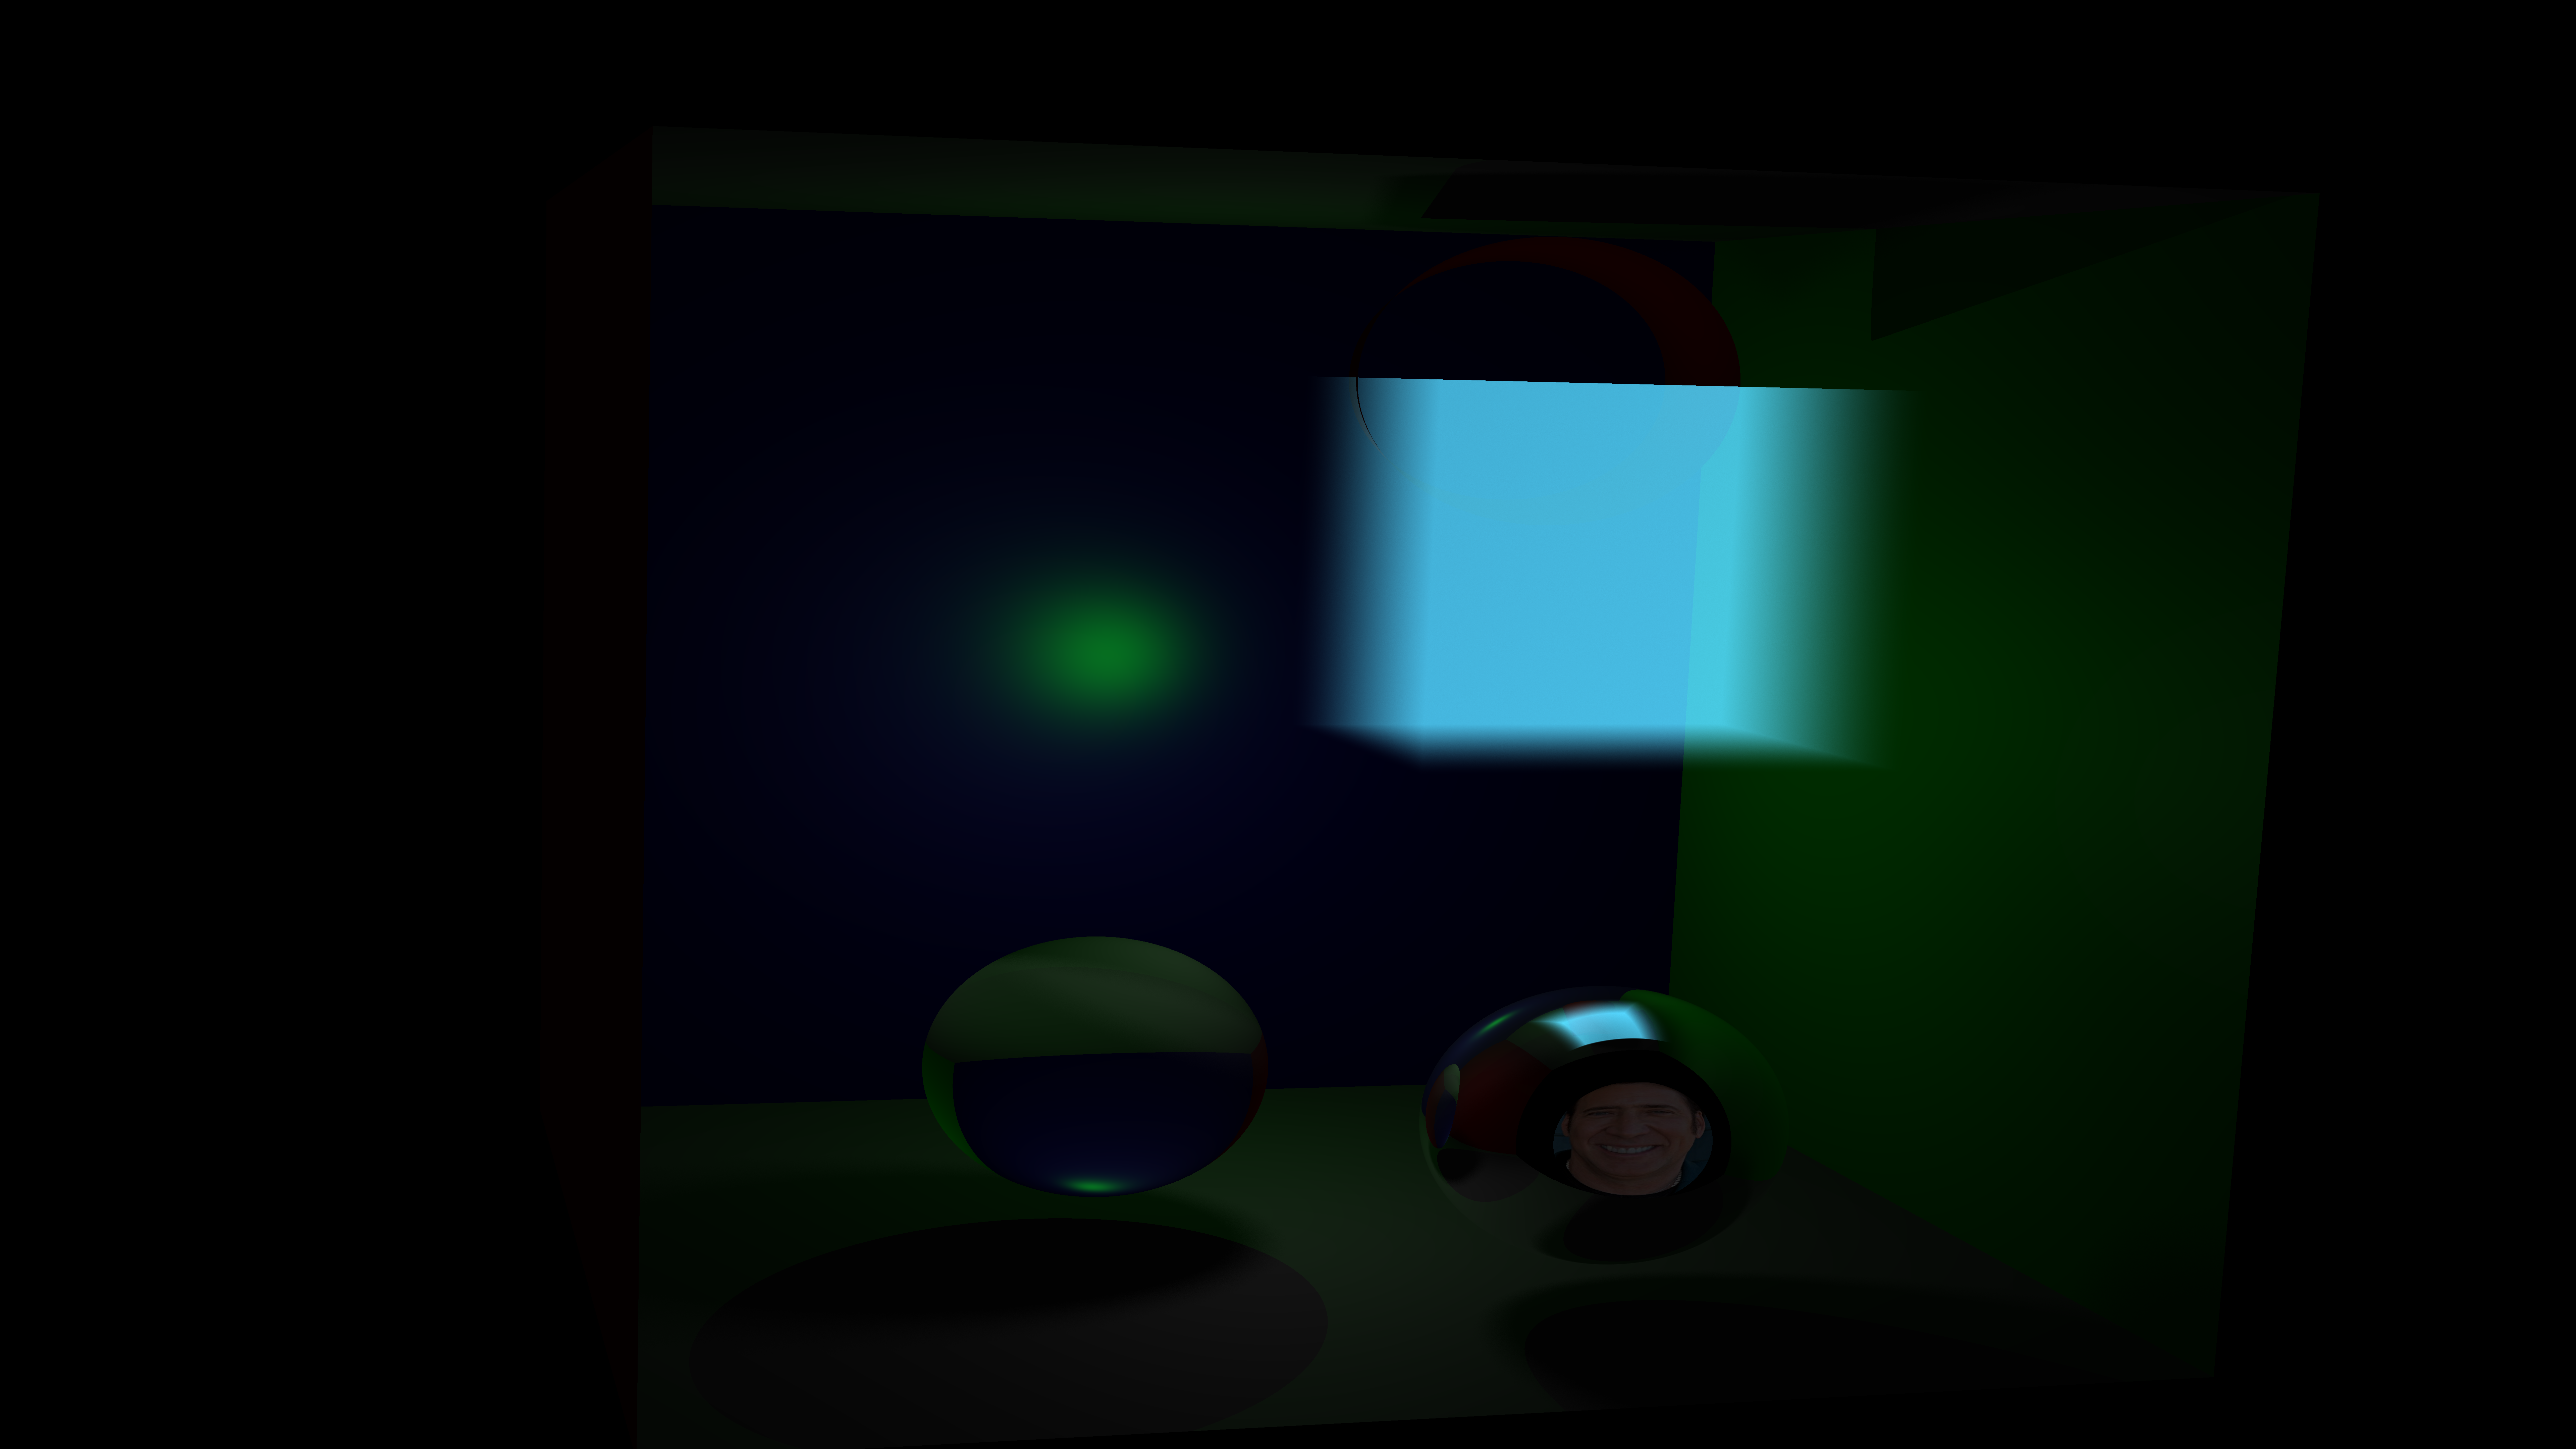
\includegraphics[scale=0.05]{color.png}
\end{center}
La semaine suivante, j'ai passé mon temps à suivre la ressource en ligne de \href{https://www.scratchapixel.com/lessons/3d-basic-rendering/volume-rendering-for-developers/intro-volume-rendering.html}{Scratchapixel}. Pierre m'a envoyé cette ressource pour que puisse bien comprendre les différentes équations reliés à l'illumination, le \textit{scattering} et le \textit{Ray Marching}. J'ai réussi à implémenter le \textit{Ray Marching} sans aucune diffculté. Cependant, l'implémentation les calculs d'illumination et de \textit{scattering} on été compliqué pour quelques raisons. Premièrement, ce sont des concepts un peu plus avancé. Deuxièmement, il fallait modifier la structure de code légèrement pour permettre certains comportements ce qui à été plus difficile qu'anticipé. \\\\
En ce moment je pense étre légèrement en retard sur mon échéancier, malgré le fait que j'ai une première version du \textit{Ray Marcher}. Lors de la semaine de lecture je vais continuer de travailler sur le \textit{Ray Marcher} et les équations associés.
\end{document}
